\documentclass[10pt]{article}
\usepackage[margin=18mm]{geometry}
\usepackage{graphicx,booktabs,array,hyperref}
\hypersetup{colorlinks=true,urlcolor=blue}
\setlength{\parindent}{0pt}\setlength{\parskip}{5pt}
\begin{document}
\section*{Structural closure panel: degree 4}
Run: \texttt{structural-20261023-02}. Experiments 2026-10-23; report 2026-10-25.

The frozen panel has 96 commands and 1152 rows: $n=13,19,23,31$,
$\ell=2,3,4$, prefix/geometric/trace-zero geometric/random bases, two recorded
base replicates and four public target draws. Prefix replicate 1 is a duplicate;
144 rows are excluded from the primary table.
Three formulations run: chained S3, direct S4, symmetric product-space S4.

Limits: degree-4 closure, 30,000 columns, 12 GiB address space, 900 seconds
per command. This shared host earns L0: timings are diagnostic only. The hybrid
extraction has an input-degree floor, which reaches six for direct S4. These
are not equal-degree or whole-query speed measurements.

There are 304 completed direct/symmetric pairs among
336 distinct input queries. The remaining 32 are unpaired, not zero-cost.
Symmetric solver work is lower in 0 pairs,
higher in 304, equal in 0.
Recorded ratios range 13.37 to 1.65e+04.
Independent direct point enumeration checks every completed answer; the audit
reports 923 complete extractions and zero failures.

\begin{center}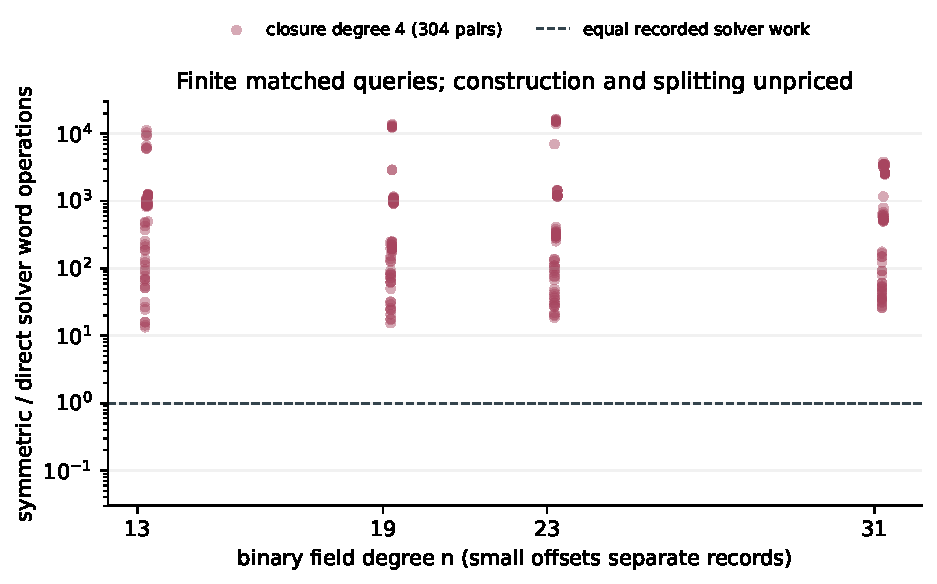
\includegraphics[width=.96\linewidth]{solver-words.pdf}\end{center}

For the completed symmetric queries, 8100 algebraic
roots produced 4 verified x-multisets;
8096 roots failed splitting or signed lifting.
Construction, splitting and physical conversion are not priced in solver words.
No end-to-end DLP cost, rho ratio, scaling law or external-CAS speed claim is made.

Raw rows: \path{../../runs/structural-20261023-02/cell-*/rows.jsonl}.
The native recomputation is \path{examples/ic_campaign_report_data.rs};
plot values are \path{../../report-data.json}. The frozen protocol, controls,
input/binary hashes, cap refusals and setup failures remain in the study.

\end{document}
